\documentclass{article}
\usepackage[margin=1in]{geometry}
\usepackage{amsmath}
\usepackage{amssymb}
\usepackage{amsthm}
\usepackage{bm}
\usepackage{hyperref}
\usepackage{graphicx}
\usepackage{caption}
\usepackage{listings}
\usepackage{xcolor}
\usepackage{float}
\usepackage{booktabs}
\usepackage{longtable}
\usepackage{multirow}
\usepackage{placeins}
\graphicspath{{figures/}}

% Code style
\lstdefinestyle{code}{
  basicstyle=\ttfamily\small,
  numbers=left,
  numberstyle=\tiny,
  numbersep=8pt,
  keywordstyle=\color{blue},
  commentstyle=\color{teal!70!black},
  stringstyle=\color{orange!70!black},
  showstringspaces=false,
  breaklines=true,
  frame=single,
  framerule=0.3pt,
  rulecolor=\color{black!15}
}
\lstset{style=code}

\title{Tool and Function Calling: Mechanisms, Hybrid Architectures, and Ecosystem Integration}
\author{}
\date{\today}

\begin{document}
\maketitle

\section{Function Calling Mechanisms (OpenAI, Anthropic)}
\subsection{Pipeline overview}
Function calling converts free-form prompts into structured requests to external tools. Figure~\ref{fig:function_pipeline_en} shows the end-to-end loop: the LLM parses the user request, emits JSON arguments, the router validates schema and dispatches the target function, tool runtimes execute, and responses are returned either to the model for post-processing or directly to the user.
\begin{figure}[H]
  \centering
  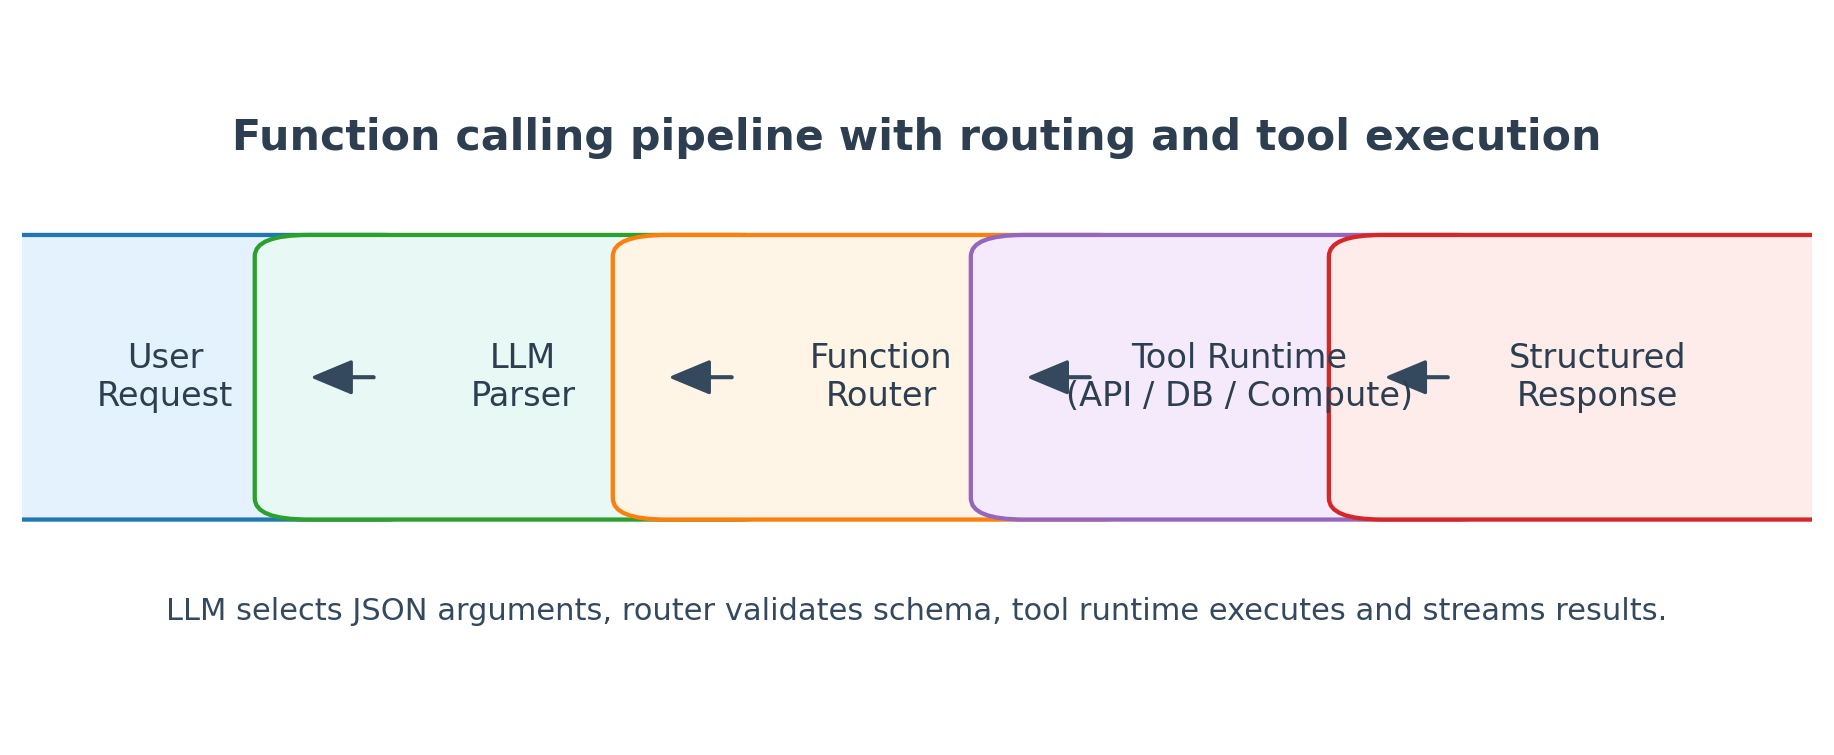
\includegraphics[width=0.9\textwidth]{function_calling_pipeline.png}
  \caption{Function calling pipeline with parsing, routing, tool execution, and structured responses.}
  \label{fig:function_pipeline_en}
\end{figure}

\subsection{Comparing OpenAI and Anthropic}
\begin{longtable}{p{3.5cm}p{5cm}p{5cm}}
\toprule
Aspect & OpenAI Function Calling & Anthropic Tool Use \\
\midrule
Interface & \texttt{functions} array with JSON Schema definitions; multi-function selection & \texttt{tools} with \texttt{input\_schema}; supports cache directives and tool metadata \\
Model output & \texttt{tool\_calls} list containing names and argument payloads; may return many at once & Message stream embeds \texttt{tool\_use} and \texttt{tool\_result} blocks for streaming interactions \\
Control flow & Model may request \texttt{none}; client decides whether to loop or finalize & Recommended tool loop: tool use \textrightarrow{} result \textrightarrow{} next reasoning step \\
Error handling & Client surfaces exceptions back to the conversation for retries & Tool results can include status/error fields that the model interprets during follow-up steps \\
Safety & Enforced via function allow-lists, schema validation, delegated approval layers & Supports \texttt{max\_tool\_outputs}, policy prompts, and tool-specific guardrails \\
\bottomrule
\end{longtable}

\subsection{OpenAI example}
\begin{lstlisting}[language=Python,caption={Calling an external weather API via OpenAI function calling}]
from openai import OpenAI
import requests

client = OpenAI(api_key="sk-...")

functions = [
    {
        "name": "get_weather",
        "description": "Retrieve weather data for a city",
        "parameters": {
            "type": "object",
            "properties": {
                "city": {"type": "string"},
                "unit": {"type": "string", "enum": ["celsius", "fahrenheit"]},
            },
            "required": ["city"],
        },
    }
]

def get_weather(city: str, unit: str = "celsius") -> str:
    resp = requests.get("https://wttr.in", params={"format": "j1", "q": city}, timeout=10)
    data = resp.json()
    temp = data["current_condition"][0]["temp_C" if unit == "celsius" else "temp_F"]
    return f"The temperature in {city} is {temp}°{unit[0].upper()}."

messages = [{"role": "user", "content": "How cold is it in Reykjavik right now?"}]
first = client.chat.completions.create(
    model="gpt-4o-mini",
    messages=messages,
    functions=functions,
)

tool_call = first.choices[0].message.tool_calls[0]
args = tool_call.function.arguments
tool_response = get_weather(args["city"], args.get("unit", "celsius"))

messages.extend([
    first.choices[0].message,
    {"role": "tool", "tool_call_id": tool_call.id, "name": "get_weather", "content": tool_response},
])

final = client.chat.completions.create(model="gpt-4o-mini", messages=messages)
print(final.choices[0].message.content)
\end{lstlisting}

\section{ReAct + Tool + Memory Hybrid Architecture}
\subsection{Reason-act loops with persistent state}
ReAct chains combine step-by-step reasoning, tool invocation, and observation logging. When paired with structured memory layers, agents maintain situational awareness across long tasks:
\begin{itemize}
  \item \textbf{Thought:} Determine whether another tool call is needed and plan the action.
  \item \textbf{Action:} Trigger function calls, plugins, or custom handlers.
  \item \textbf{Observation:} Parse tool output, update working context, and decide on next steps.
  \item \textbf{Memory write:} Persist key facts into short-term conversational buffers and long-term vector stores.
\end{itemize}

\subsection{Memory tiers}
\begin{itemize}
  \item Working memory stores recent dialogue turns, tool traces, and temporary variables.
  \item Long-term memory captures user preferences, previous projects, and domain knowledge in vector DBs or knowledge graphs.
  \item Episodic memory tracks task timelines, checkpoints, and artifacts for reproducibility.
\end{itemize}

\subsection{Governance safeguards}
\begin{itemize}
  \item Filter memory writes for PII or sensitive data before persistence.
  \item Employ guard models to inspect tool outputs and proposed actions, blocking risky behavior.
  \item Apply rate limits and idempotency tokens on critical tools (payments, infrastructure control).
\end{itemize}

\section{WebAgent / OS-Agent Implementation Strategies}
\subsection{Hybrid stack}
Web and OS agents rely on distinct tool stacks yet share memory and governance components. Figure~\ref{fig:hybrid_agent_stack_en} depicts a typical arrangement with controllers, tooling interfaces, state caches, shared memory, and policy enforcement.
\begin{figure}[H]
  \centering
  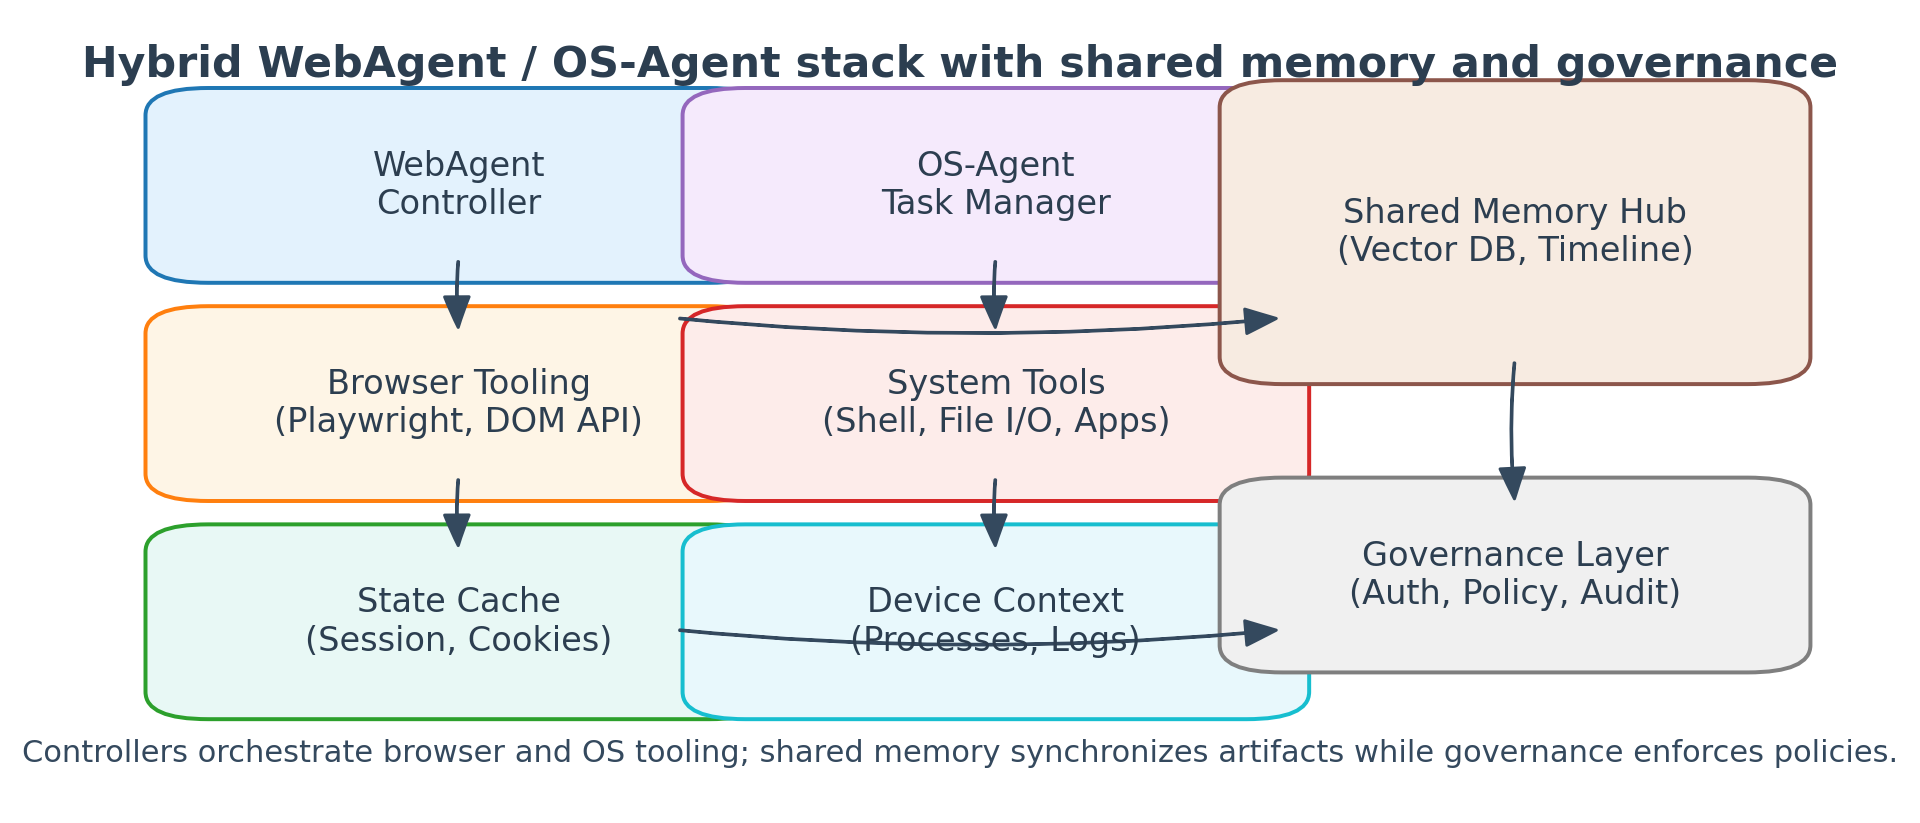
\includegraphics[width=0.9\textwidth]{hybrid_agent_stack.png}
  \caption{Hybrid WebAgent/OS-Agent stack with shared memory and governance.}
  \label{fig:hybrid_agent_stack_en}
\end{figure}

\subsection{WebAgent components}
\begin{itemize}
  \item \textbf{Browser automation:} Playwright, Selenium, or puppeteer for DOM interaction, keyboard/mouse simulation.
  \item \textbf{Page understanding:} HTML parsing, screenshot captioning, layout analysis, or multimodal embeddings.
  \item \textbf{Session management:} Persist cookies, local storage, and history to enable multi-step workflows.
  \item \textbf{Safety filters:} Block known malicious URLs, sanction scripts, and enforce domain allow-lists.
\end{itemize}

\subsection{OS-Agent components}
\begin{itemize}
  \item \textbf{System tools:} Shell commands, PowerShell, AppleScript, file system operations, process control.
  \item \textbf{Context capture:} Access process lists, system logs, telemetry dashboards, and hardware status.
  \item \textbf{Task manager:} Track job states, roll back changes, and recover after exceptions or system reboots.
  \item \textbf{Policy engine:} Handle authentication, privilege escalation, and create immutable audit trails.
\end{itemize}

\subsection{Shared memory and coordination}
Agents sync artifacts (documents, screenshots, runtime logs) via a shared vector hub or timeline store, enabling workflows that span browsers and operating systems.

\section{External API and Plugin Integration}
\subsection{Plugin landscape}
\begin{itemize}
  \item \textbf{Communication APIs:} Slack, Teams, Gmail, or SMS gateways for notifications and approvals.
  \item \textbf{Business systems:} CRM/ERP (Salesforce, HubSpot), issue trackers (Jira, Linear), analytics (Looker, Tableau).
  \item \textbf{Data services:} SQL/NoSQL databases, data lakes, vector stores, knowledge graphs, proprietary services.
\end{itemize}

\subsection{Integration patterns}
\begin{itemize}
  \item Direct function registration where the LLM invokes plugins via standard schemas.
  \item Proxy orchestrators that validate requests, handle retries, and enforce quotas before hitting APIs.
  \item Workflow engines (Temporal, Airflow, Camunda) to combine automated steps with human approval gates.
\end{itemize}

\subsection{Security posture}
\begin{itemize}
  \item Use OAuth2/JWT with least-privilege scopes; rotate tokens and secrets automatically.
  \item Capture audit logs for every tool invocation, including parameters and response hashes.
  \item Sanitize and redact sensitive responses before they enter long-term memory or external channels.
\end{itemize}

\subsection{Plugin example}
\begin{lstlisting}[language=Python,caption={Writing a research note to Notion through the public API}]
import os
import requests

NOTION_TOKEN = os.environ["NOTION_TOKEN"]
DATABASE_ID = os.environ["NOTION_DB"]

headers = {
    "Authorization": f"Bearer {NOTION_TOKEN}",
    "Notion-Version": "2022-06-28",
    "Content-Type": "application/json",
}

payload = {
    "parent": {"database_id": DATABASE_ID},
    "properties": {
        "Title": {"title": [{"text": {"content": "Geothermal Inversion Summary"}}]},
        "Status": {"select": {"name": "Draft"}},
    },
    "children": [
        {"object": "block", "type": "paragraph", "paragraph": {"rich_text": [
            {"type": "text", "text": {"content": "Draft prepared by OS-Agent after log analysis."}}
        ]}}
    ],
}

resp = requests.post("https://api.notion.com/v1/pages", headers=headers, json=payload, timeout=15)
resp.raise_for_status()
\end{lstlisting}

\section*{Operational recommendations}
\begin{itemize}
  \item Standardize JSON Schemas for every tool, document side effects, and generate synthetic tests for regression coverage.
  \item Log tool inputs/outputs with correlation IDs to support replay, debugging, and safe re-execution.
  \item Introduce human approval checkpoints or automated policy evaluators for high-impact actions.
  \item Conduct regular red-team exercises to verify that governance layers catch prompt injection and privilege escalation attempts.
\end{itemize}

\section*{Further reading}
\begin{itemize}
  \item OpenAI. ``Function Calling and JSON Mode.'' Developer Blog, 2023.
  \item Anthropic. ``Claude Tool Use.'' Technical Guide, 2024.
  \item Yao et al. ``ReAct: Synergizing Reasoning and Acting in Language Models.'' ICLR, 2023.
  \item Qin et al. ``WebArena: A Realistic Web Environment for Building Autonomous Agents.'' NeurIPS, 2023.
  \item Xu et al. ``TaskMatrix.AI: Enabling LLMs to Master 1600+ Real-World APIs.'' arXiv, 2023.
\end{itemize}

\end{document}

